\documentclass[conference]{IEEEtran}
\IEEEoverridecommandlockouts
\usepackage{amsmath,amssymb,amsfonts}
\usepackage{algorithmic}
\usepackage{graphicx}
\usepackage{textcomp}
\usepackage{xcolor}
\usepackage{subcaption}
\usepackage[style=numeric,backend=biber]{biblatex}
\addbibresource{references.bib}
\begin{document}

\title{Deeper Networks for Image Classification}

\author{\IEEEauthorblockN{Alexander Sworski}
\IEEEauthorblockA{\textit{ECS795P – Deep Learning and Computer Vision} \\
\textit{School of Electronic Engineering and Computer Science - Department of Computer Science} \\ {M.Sc. Artificial Intelligence}  \\ 
\textit{Queen Mary University}\\
London, United Kingdom \\
a.sworski@se21.qmul.ac.uk \\
210456914}
}

\maketitle

\begin{abstract}
This paper represents a comparison between different Convolutional Neural Networks. In particular, the models GoogLeNet, VGG-16 and ResNet are compared on different datasets, such as MNIST and Cifar10.
\end{abstract}

\begin{IEEEkeywords}
GoogLeNet, ResNet, VGG-16, MNIST, Image Classification, Deep Learning
\end{IEEEkeywords}

\section{Introduction}
This document is a model and instructions for \LaTeX.
%Please observe the conference page limits. 

\section{Literature Review}

\subsection{Neural Network models}
\subsubsection{GoogLeNet}
GoogLeNet, was initially developed as a submission for the ImageNet Large-Scale Visual Recognition Challenge 2014, which it won. The main hallmark of this model is the improved utilisation of the computing resources inside the network. It has 12 times fewer parameters than the winner of 2012 (AlexNet) but performs significantly better. \cite{szegedy_going_2014}
This model first introduced the idea of an inception module, which can be seen in Figure \ref{fig:x inception module 5x5}.
A second version of the model was published a year later, which then introduced an improved inception module, which can been seen in Figure \ref{fig:x inception module 3x3}.
This new version reduced computational costs, as bigger convolutions are disproportionately more expensive. Using two 3x3 convolutions instead it computationally less expensive while improving the performance.
Although there are is also a V3 and V4 of GoogLeNet, for this paper, the V2 Inception has been used.
In total the model has 22 layers.
\begin{figure}[!htbp]
     \centering
     \begin{subfigure}[b]{0.25\textwidth}
         \centering
         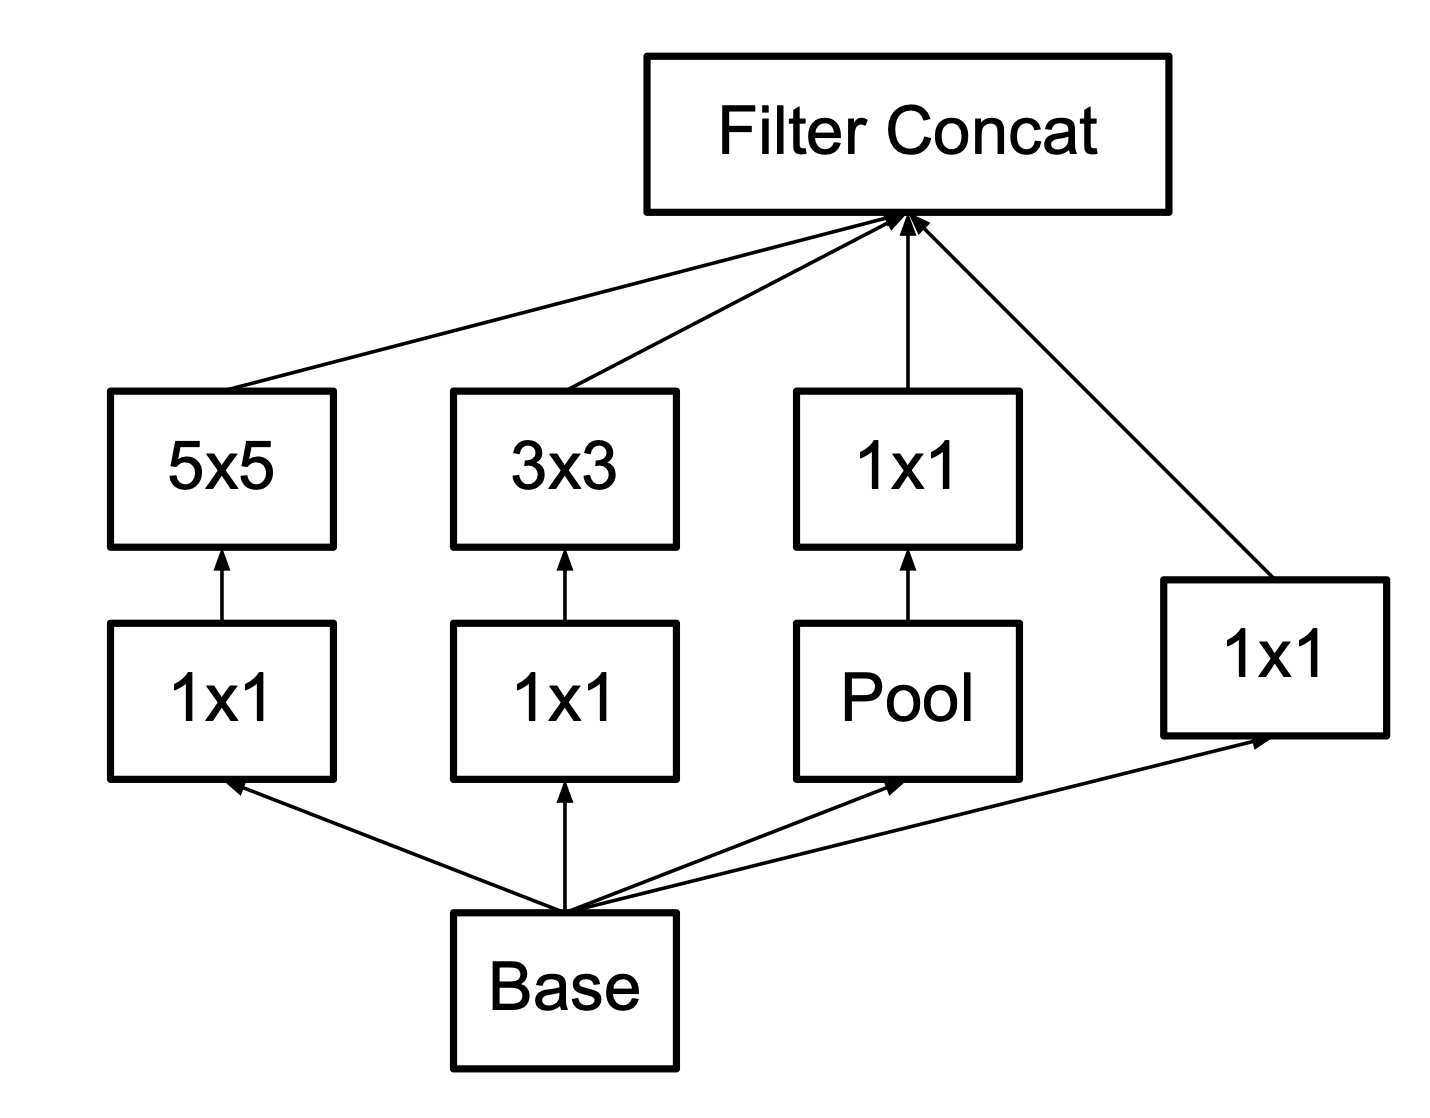
\includegraphics[width=\textwidth]{img/inceptionv1.png}
         \caption{Original Inception module \cite{szegedy_going_2014}}
         \label{fig:x inception module 5x5}
     \end{subfigure}
     \hfill
     \begin{subfigure}[b]{0.22\textwidth}
         \centering
         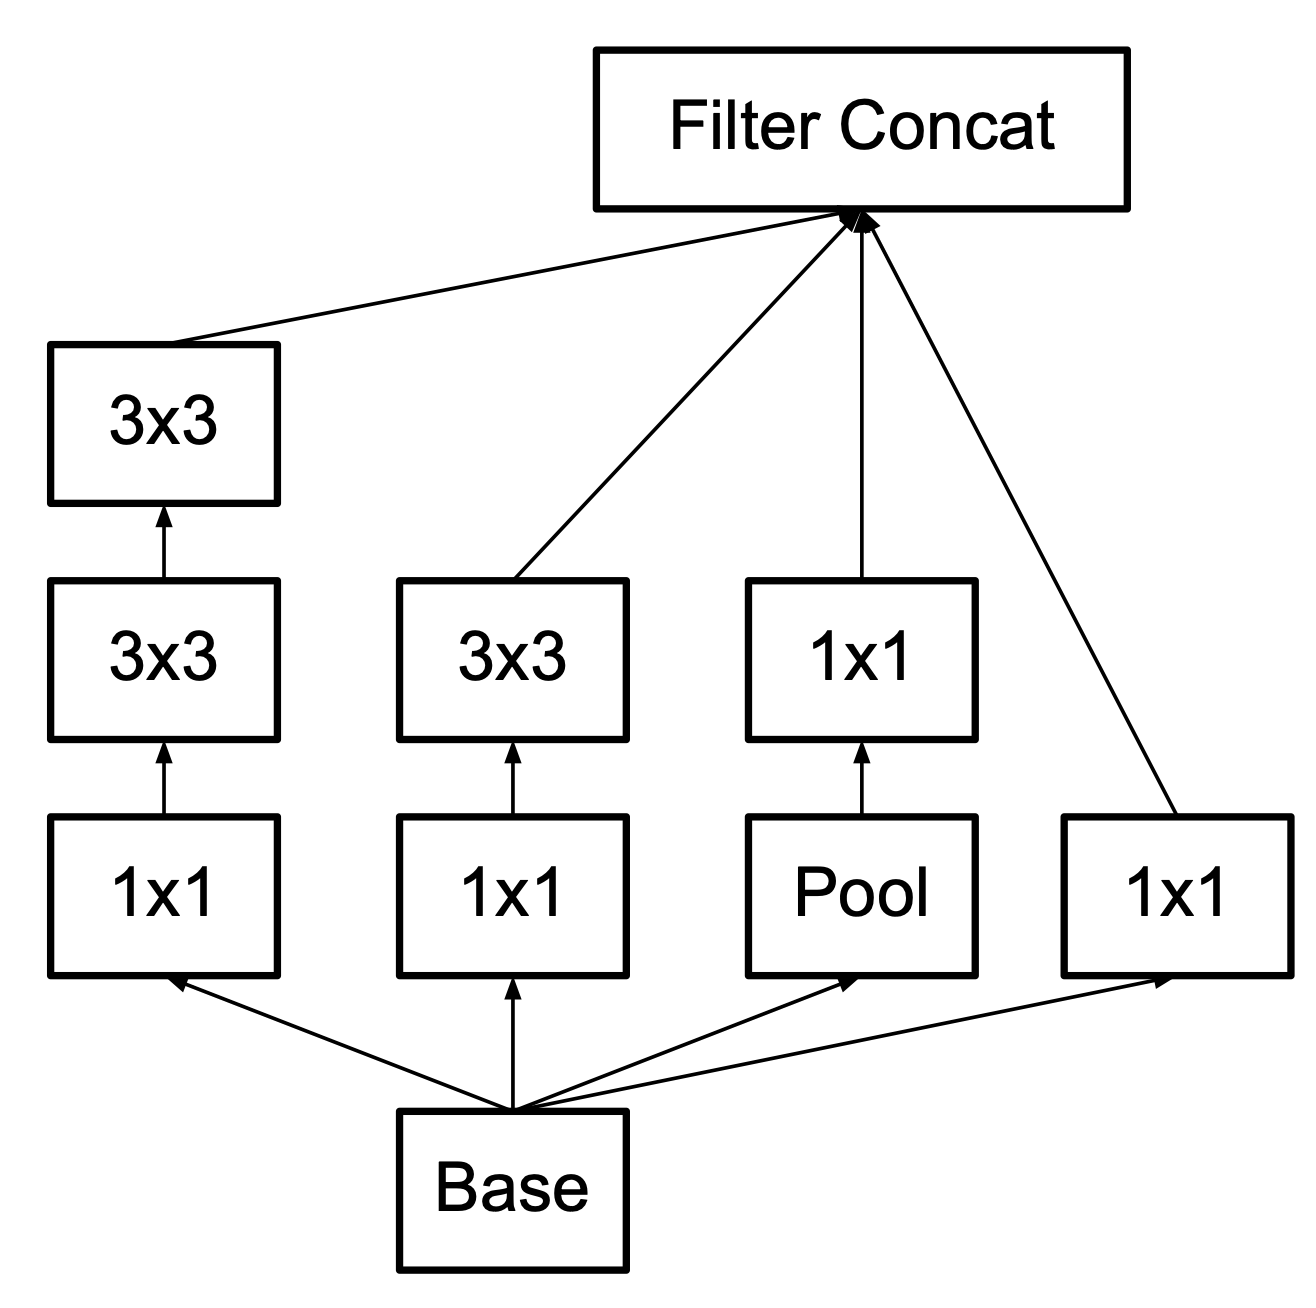
\includegraphics[width=\textwidth]{img/incetionv2.png}
         \caption{V2 Inception module \cite{szegedy_rethinking_2015}}
         \label{fig:x inception module 3x3}
     \end{subfigure}
        \caption{Three simple graphs}
        \label{fig:three graphs}
\end{figure}

\subsubsection{VGG-16}
VGG-16, is the biggest of the models used in this paper (Figure \ref{fig:x mode size}).
It also has been developed as a submission for the ImageNet Challenge, in which it won first and second place for the localization and classification tracks, respectively.
It consists out of 16 layers and uses only 3x3 convolutions. Although it has fewer layers than GoogLeNet, each layer is computationally more complex. Ultimately, this model resulted in better scores then the GoogLeNet V1 \cite{simonyan_very_2015}.

\begin{figure}[!htbp]
    \centering
    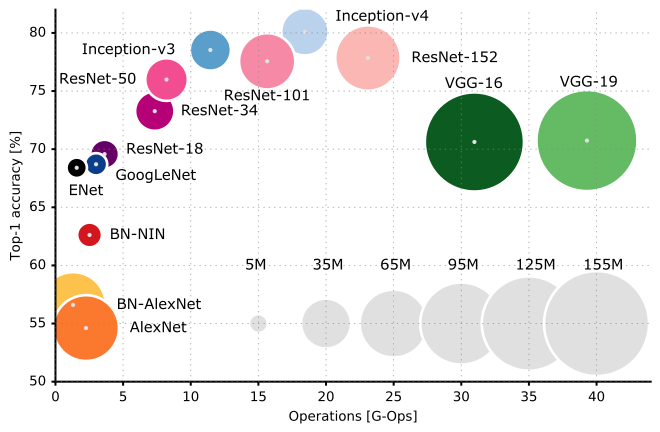
\includegraphics[scale=0.35]{img/model_sizes.png}
    \caption{top-1 one-crop accuracy versus amount of operations required (circle size represents the amount of parameters)}
    \label{fig:x mode size}
\end{figure}

\subsubsection{ResNet}
ResNet, has the highest amount of layers. While there are multiple versions, for this paper a 50 layer version has been chosen.
\begin{figure}[!htbp]
    \centering
    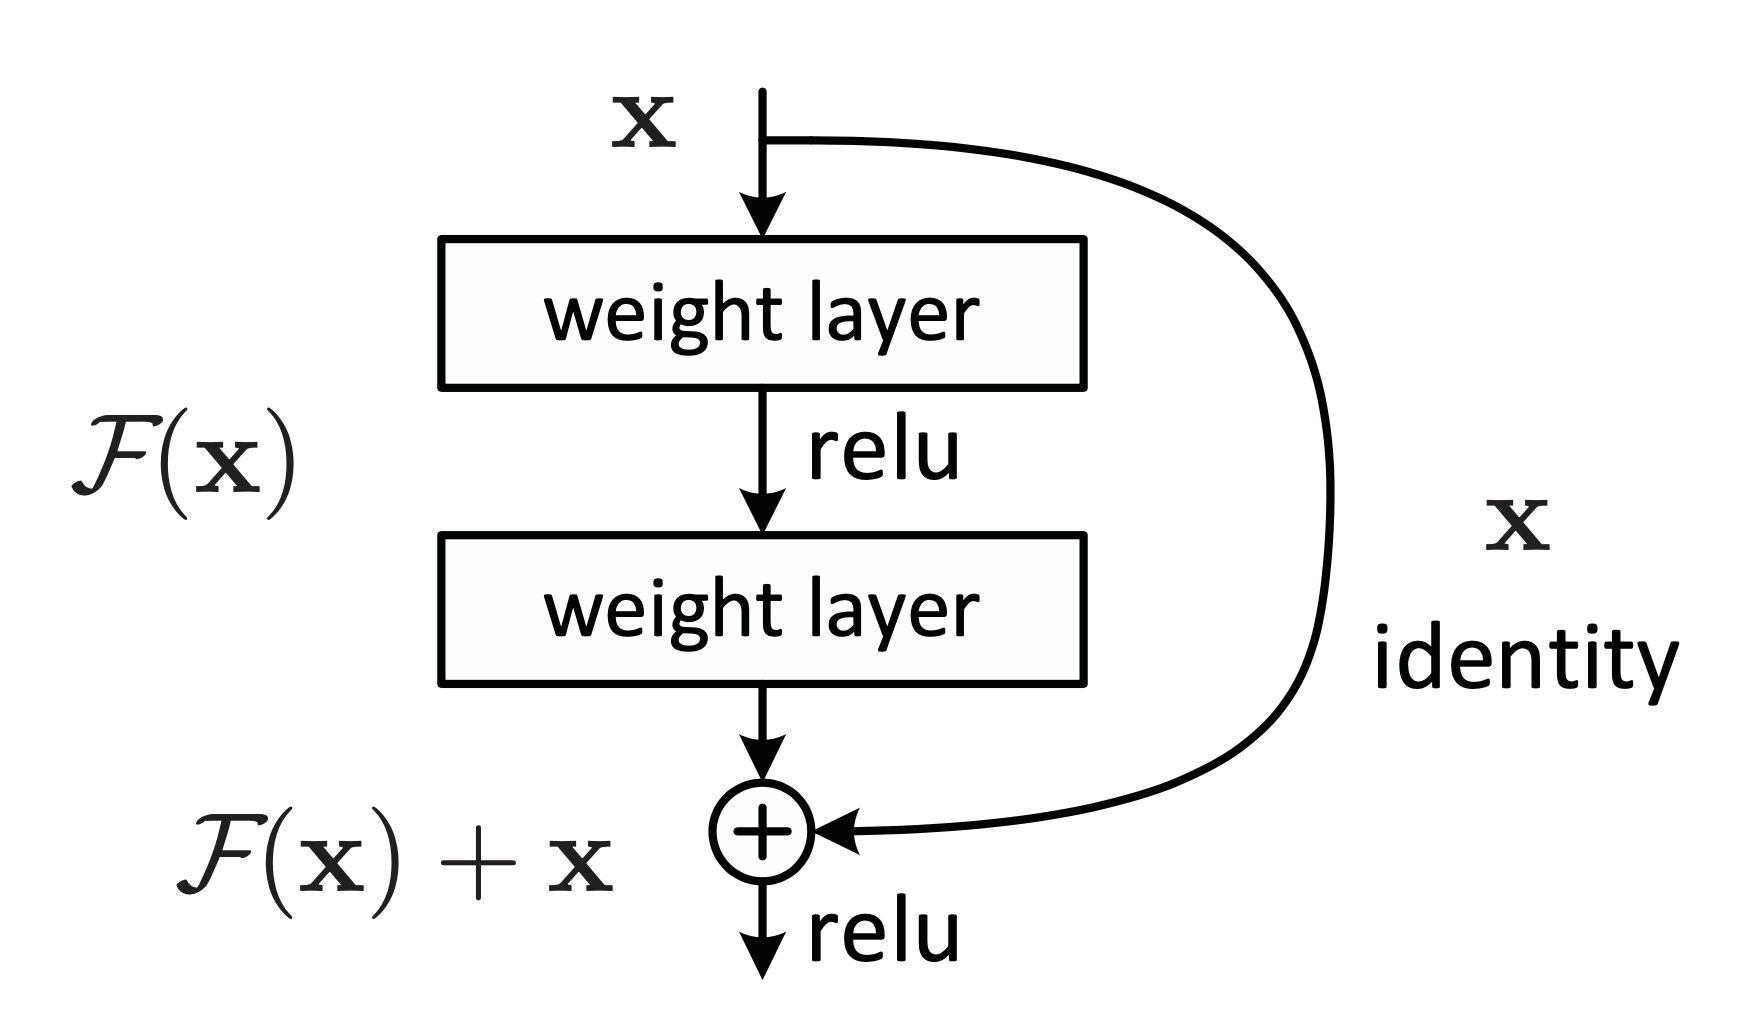
\includegraphics[scale=0.2]{img/residual block.png}
    \caption{Residual learning: a building block \cite{he_deep_2015}}
    \label{fig:x resblock}
\end{figure}
In Figure \ref{fig:x mode size} it can be observed, that the model size is in between GoogLeNet and VGG-16, yet the best result can be expected according to this comparison.
ResNet has been build with the goal of easing the training of deep networks. The network design is based on the concept of chaining multiple residual learning block on a row. One residual learning block can be seen in Figure \ref{fig:x resblock}. \cite{he_deep_2015}


\subsection{Image datasets}
\subsubsection{MNIST}
The MNIST database contains 70,000 28x28 black and white images. 60,000 images are for training and 10,000 images for testing. The images' portrait handwritten numbers from 0 to 9. \cite{yann_lecun_mnist_nodate} Examples of the classes can be seen in Figure \ref{fig:x MNIST image samples}.
\begin{figure}[!htbp]
    \centering
    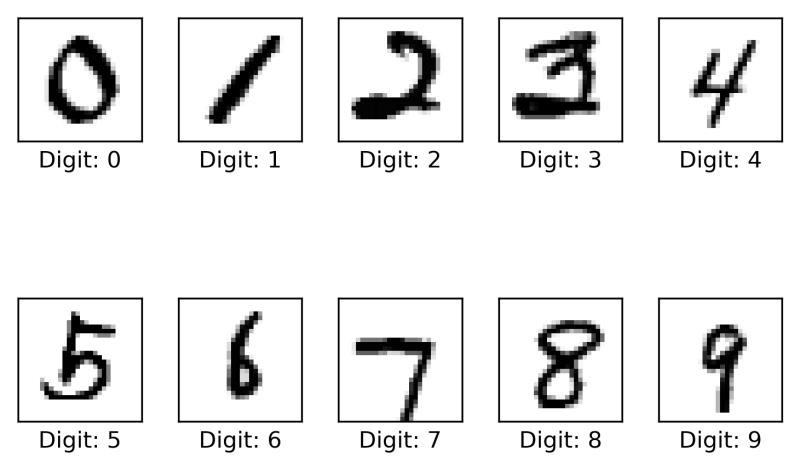
\includegraphics[scale=0.35]{img/mnist_sample.jpeg}
    \caption{Cifar10 image samples \cite{noauthor_convolutional_nodate}}
    \label{fig:x MNIST image samples}
\end{figure}
\subsubsection{Cifar10}
The CIFAR-10 dataset consists of 60000 32x32 colour images in 10 classes, with 6000 images per class. There are 50000 training images and 10000 test images. The classes are mutually exclusive.\cite{noauthor_cifar-10_nodate} Examples of the classes can be seen in Figure \ref{fig:x Cifar10 image samples}.
\begin{figure}[!htbp]
    \centering
    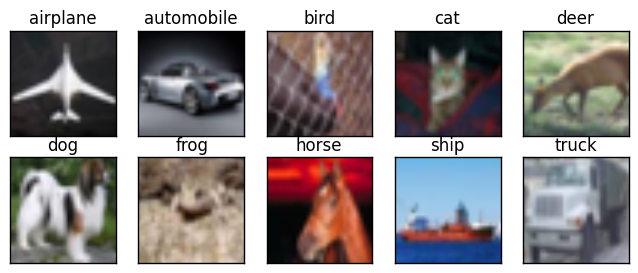
\includegraphics[scale=0.45]{img/cifar_10_sample.png}
    \caption{Cifar10 image samples \cite{noauthor_fig_nodate}}
    \label{fig:x Cifar10 image samples}
\end{figure}

\section{Implementation}
In the first subsection \ref{IM} the implementation of the models using the framework Keras will be explained.
The the subsection \ref{ID}, it will be explained how the datasets have been made compatible with the models.
\subsection{Model implementation}\label{IM}
\subsubsection{GoogLeNet}
\subsubsection{ResNet}
\subsubsection{VGG-16}
\subsection{The Datasets}\label{ID}

The dataset used in this paper, both have a resolution of 28x28 pixels. On top, the Cifar10 dataset has 3 colour channels, while the MNIST dataset only has one grey channel.
This represents an issue, as the Neural Networks have initially been designed to work with the Microsoft ImageNet dataset. This dataset has 3 colour channels and a resolution of 224x224 pixels.
The goal was to not change the input of the models, as this would have significant implications for the layers following, resulting in a significant change in the model design.
Therefore, the datasets have been altered as follows to fit the input dimensions of the models.

\subsubsection{MNIST dataset alterations}
The MNIST dataset originally has the shape (28,28,1), while our models required an input shape of (224,224,3). 
In order to change the dimensionality, the OpenCV library has been used. Using OpenCV, the image has been interpolated to fit the 224x224 image size. 
Afterwards, the image has been stacked three times, so that we obtain our three channel input. Although, there is the OpenCV function \verb|cv2.cvtColor(src, cv2.COLOR_GRAY2RGB)|, 
which can convert from greyscale to RGB, the results are not different from our stacked layers. 
This is due to the unique properties the MNIST dataset has. Using the stacked layers, is computational much more lightweight.

\subsubsection{Cifar10 dataset alterations}
The Cifar10 dataset is already in RGB. Therefore, we do not need to convert it into a different colour space. 
Therefore, this dataset has been interpolated from the shape (28,28,3) to (224,224,3) using the OpenCV library.

\subsection{Abbreviations and Acronyms}\label{AA}
Define abbreviations and acronyms the first time they are used in the text, 
even after they have been defined in the abstract. Abbreviations such as 
IEEE, SI, MKS, CGS, ac, dc, and rms do not have to be defined. Do not use 
abbreviations in the title or heads unless they are unavoidable.

\subsection{Units}
\begin{itemize}
\item Use either SI (MKS) or CGS as primary units. (SI units are encouraged.) English units may be used as secondary units (in parentheses). An exception would be the use of English units as identifiers in trade, such as ``3.5-inch disk drive''.
\item Avoid combining SI and CGS units, such as current in amperes and magnetic field in oersteds. This often leads to confusion because equations do not balance dimensionally. If you must use mixed units, clearly state the units for each quantity that you use in an equation.
\item Do not mix complete spellings and abbreviations of units: ``Wb/m\textsuperscript{2}'' or ``webers per square meter'', not ``webers/m\textsuperscript{2}''. Spell out units when they appear in text: ``. . . a few henries'', not ``. . . a few H''.
\item Use a zero before decimal points: ``0.25'', not ``.25''. Use ``cm\textsuperscript{3}'', not ``cc''.)
\end{itemize}

\subsection{Equations}
Number equations consecutively. To make your 
equations more compact, you may use the solidus (~/~), the exp function, or 
appropriate exponents. Italicize Roman symbols for quantities and variables, 
but not Greek symbols. Use a long dash rather than a hyphen for a minus 
sign. Punctuate equations with commas or periods when they are part of a 
sentence, as in:
\begin{equation}
a+b=\gamma\label{eq}
\end{equation}

Be sure that the 
symbols in your equation have been defined before or immediately following 
the equation. Use ``\eqref{eq}'', not ``Eq.~\eqref{eq}'' or ``equation \eqref{eq}'', except at 
the beginning of a sentence: ``Equation \eqref{eq} is . . .''

\subsection{\LaTeX-Specific Advice}

Please use ``soft'' (e.g., \verb|\eqref{Eq}|) cross references instead
of ``hard'' references (e.g., \verb|(1)|). That will make it possible
to combine sections, add equations, or change the order of figures or
citations without having to go through the file line by line.

Please don't use the \verb|{eqnarray}| equation environment. Use
\verb|{align}| or \verb|{IEEEeqnarray}| instead. The \verb|{eqnarray}|
environment leaves unsightly spaces around relation symbols.

Please note that the \verb|{subequations}| environment in {\LaTeX}
will increment the main equation counter even when there are no
equation numbers displayed. If you forget that, you might write an
article in which the equation numbers skip from (17) to (20), causing
the copy editors to wonder if you've discovered a new method of
counting.

{\LaTeX} can't read your mind. If you assign the same label to a
subsubsection and a table, you might find that Table I has been cross
referenced as Table IV-B3. 

{\LaTeX} does not have precognitive abilities. If you put a
\verb|\label| command before the command that updates the counter it's
supposed to be using, the label will pick up the last counter to be
cross referenced instead. In particular, a \verb|\label| command
should not go before the caption of a figure or a table.

Do not use \verb|\nonumber| inside the \verb|{array}| environment. It
will not stop equation numbers inside \verb|{array}| (there won't be
any anyway) and it might stop a wanted equation number in the
surrounding equation.

\subsection{Some Common Mistakes}\label{SCM}
\begin{itemize}
\item The word ``data'' is plural, not singular.
\item The subscript for the permeability of vacuum $\mu_{0}$, and other common scientific constants, is zero with subscript formatting, not a lowercase letter ``o''.
\item In American English, commas, semicolons, periods, question and exclamation marks are located within quotation marks only when a complete thought or name is cited, such as a title or full quotation. When quotation marks are used, instead of a bold or italic typeface, to highlight a word or phrase, punctuation should appear outside of the quotation marks. A parenthetical phrase or statement at the end of a sentence is punctuated outside of the closing parenthesis (like this). (A parenthetical sentence is punctuated within the parentheses.)
\item A graph within a graph is an ``inset'', not an ``insert''. The word alternatively is preferred to the word ``alternately'' (unless you really mean something that alternates).
\item Do not use the word ``essentially'' to mean ``approximately'' or ``effectively''.
\item In your paper title, if the words ``that uses'' can accurately replace the word ``using'', capitalise the ``u''; if not, keep using lower-cased.
\item Be aware of the different meanings of the homophones ``affect'' and ``effect'', ``complement'' and ``compliment'', ``discreet'' and ``discrete'', ``principal'' and ``principle''.
\item Do not confuse ``imply'' and ``infer''.
\item The prefix ``non'' is not a word; it should be joined to the word it modifies, usually without a hyphen.
\item There is no period after the ``et'' in the Latin abbreviation ``et al.''.
\item The abbreviation ``i.e.'' means ``that is'', and the abbreviation ``e.g.'' means ``for example''.
\end{itemize}
An excellent style manual for science writers is \cite{}.

\subsection{Authors and Affiliations}
\textbf{The class file is designed for, but not limited to, six authors.} A 
minimum of one author is required for all conference articles. Author names 
should be listed starting from left to right and then moving down to the 
next line. This is the author sequence that will be used in future citations 
and by indexing services. Names should not be listed in columns nor group by 
affiliation. Please keep your affiliations as succinct as possible (for 
example, do not differentiate among departments of the same organisation).

\subsection{Identify the Headings}
Headings, or heads, are organisational devices that guide the reader through 
your paper. There are two types: component heads and text heads.

Component heads identify the different components of your paper and are not 
topically subordinate to each other. Examples include Acknowledgments and 
References and, for these, the correct style to use is ``Heading 5''. Use 
``figure caption'' for your Figure captions, and ``table head'' for your 
table title. Run-in heads, such as ``Abstract'', will require you to apply a 
style (in this case, italic) in addition to the style provided by the drop 
down menu to differentiate the head from the text.

Text heads organise the topics on a relational, hierarchical basis. For 
example, the paper title is the primary text head because all subsequent 
material relates and elaborates on this one topic. If there are two or more 
sub-topics, the next level head (uppercase Roman numerals) should be used 
and, conversely, if there are not at least two sub-topics, then no subheads 
should be introduced.

\subsection{Figures and Tables}
\paragraph{Positioning Figures and Tables} Place figures and tables at the top and 
bottom of columns. Avoid placing them in the middle of columns. Large 
figures and tables may span across both columns. Figure captions should be 
below the figures; table heads should appear above the tables. Insert 
figures and tables after they are cited in the text. Use the abbreviation 
``Fig.~\ref{fig}'', even at the beginning of a sentence.

\begin{table}[htbp]
\caption{Table Type Styles}
\begin{center}
\begin{tabular}{|c|c|c|c|}
\hline
\textbf{Table}&\multicolumn{3}{|c|}{\textbf{Table Column Head}} \\
\cline{2-4} 
\textbf{Head} & \textbf{\textit{Table column subhead}}& \textbf{\textit{Subhead}}& \textbf{\textit{Subhead}} \\
\hline
copy& More table copy$^{\mathrm{a}}$& &  \\
\hline
\multicolumn{4}{l}{$^{\mathrm{a}}$Sample of a Table footnote.}
\end{tabular}
\label{tab1}
\end{center}
\end{table}

Figure Labels: Use 8 point Times New Roman for Figure labels. Use words 
rather than symbols or abbreviations when writing Figure axis labels to 
avoid confusing the reader. As an example, write the quantity 
``Magnetization'', or ``Magnetization, M'', not just ``M''. If including 
units in the label, present them within parentheses. Do not label axes only 
with units. In the example, write ``Magnetization (A/m)'' or ``Magnetization 
\{A[m(1)]\}'', not just ``A/m''. Do not label axes with a ratio of 
quantities and units. For example, write ``Temperature (K)'', not 
``Temperature/K''.

\section*{Acknowledgment}

The preferred spelling of the word ``acknowledgment'' in America is without 
an ``e'' after the ``g''. Avoid the stilted expression ``one of us (R. B. 
G.) thanks $\ldots$''. Instead, try ``R. B. G. thanks$\ldots$''. Put sponsor 
acknowledgments in the unnumbered footnote on the first page.

\section*{References}

Please number citations consecutively within brackets \cite{}. The 
sentence punctuation follows the bracket \cite{}. Refer simply to the reference 
number, as in \cite{}---do not use ``Ref. \cite{}'' or ``reference \cite{}'' except at 
the beginning of a sentence: ``Reference \cite{} was the first $\ldots$''

Number footnotes separately in superscripts. Place the actual footnote at 
the bottom of the column in which it was cited. Do not put footnotes in the 
abstract or reference list. Use letters for table footnotes.

Unless there are six authors or more give all authors' names; do not use 
``et al.''. Papers that have not been published, even if they have been 
submitted for publication, should be cited as ``unpublished'' \cite{}. Papers 
that have been accepted for publication should be cited as ``in press'' \cite{}. 
Capitalise only the first word in a paper title, except for proper nouns and 
element symbols.

For papers published in translation journals, please give the English 
citation first, followed by the original foreign-language citation \cite{}.


\printbibliography

\end{document}
